\documentclass[12pt]{article}

\usepackage[T2A]{fontenc}
\usepackage[utf8]{inputenc}
\usepackage[serbianc]{babel}

\usepackage{amsmath}
\usepackage{amssymb}
\usepackage{braket}

\usepackage{graphicx}
\usepackage{wrapfig}
\usepackage{xcolor}
\usepackage[hidelinks]{hyperref}

\usepackage{ntheorem}
\theoremstyle{plain}
\newtheorem{teorema}{Теорема}[section]
\newtheorem{lema}{Лема}[section]
\theoremstyle{definition}
\newtheorem{definicija}{Дефиниција}[section]

%\usepackage[skip=0.7em]{parskip}
\setlength{\parskip}{0.7em}
\setlength{\parindent}{1.5em}

\title{Квантни рачунари}
\author{Андреј Топић}
\date{\today}

\begin{document}
	
	\maketitle
	\thispagestyle{empty}
	\newpage
	
	\tableofcontents
	\newpage
	
	\section{Увод}
	
	Развој модерне информатике дуго се ослањао на усавршавање класичних рачунара и Муров закон, али су научници већ крајем 20. века уочили границе таквог приступа. Кључни тренутак догодио се 1981. године када је амерички физичар Ричард Фајнман (Richard Feynman) изнео тезу да природа у својој основи није класична, већ квантна, и да, ако желимо истински да симулирамо природне процесе на нивоу атома и молекула, класични рачунари то никада неће моћи да ураде ефикасно јер се са сложеношћу система број потребних операција експоненцијално повећава.
	
	Ова идеја је поставила темеље за нову врсту рачунарства – уместо да покушавамо да „натерамо” природу да се прилагоди класичној логици нула и јединица, треба да направимо машине које директно користе законе квантне механике за свој рад.
	
	Главни разлог за развој ове технологије лежи у тзв. \textcolor{red}{„експоненцијалној баријери”} класичних рачунара. Постоје проблеми, попут факторизације веома великих бројева, где додавање само једног новог елемента дуплира тежину проблема. Квантни рачунари нуде пут ка превазилажењу ових ограничења.
	
	\section{Принцип рада}
	
	\subsection{Кубити (Qubits)}
	Основна јединица информације код квантних рачунара је \textit{кубит}. За разлику од класичног бита који може бити искључиво у стању 0 или 1, кубит може да буде у оба стања истовремено (суперпозиција) све док се не изврши мерење. Ова специфичност омогућава квантним системима да обрађују огромну количину података паралелно, што је и главни извор њихове снаге.
	
	\begin{wrapfigure}{l}{0.4\textwidth}
		\centering
		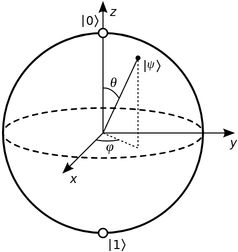
\includegraphics[width=0.4\textwidth]{./slike/bloch_sphere.png}
		\caption{Кубит приказан у виду Блохове сфере}
		\label{fig:qubit}
	\end{wrapfigure}
	
	\subsection{Суперпозиција (Superposition)}
	За разлику од класичног бита који има два могућа дискретна стања - или 0 или 1, кубит може постојати у стању које је линеарна комбинација ова два стања. Математички, ово јединствено стање $\ket{\psi}$ описујемо формулом:
	
	\begin{equation}
		\ket{\psi}=\alpha\ket{0}+\beta\ket{1}
	\end{equation}
	
	\noindent где су $\alpha$ и $\beta$ комплексни бројеви који представљају амплитуде вероватноће, при чему важи да је:
	
	\begin{equation}
		|\alpha|^2 + |\beta|^2 = 1
	\end{equation}
	
	\noindent Ово својство омогућава квантном рачунару да у једном тренутку обрађује огроман број могућности паралелно. Међутим, оног тренутка када извршимо мерење, односно када на неки начин утичемо на наш квантни систем који се налази у оквиру QPU, суперпозиција се гаси и кубит „бира” једно од два стања (0 или 1).
	
	\subsection{Уплетеност (Entanglement)}
	Уплетеност је специфичан квантни феномен где су две или више честица повезане на такав начин да деле идентично квантно стање, без обзира на њихову међусобну удаљеност; када измеримо једну честицу, тј. када јој очитамо њено квантно стање, аутоматски смо измерили и другу честицу која је повезана (уплетена) са њом. На исти начин, у контексту квантних рачунара, можемо описати и уплетеност кубита. У израчунавањима ово значи да промена стања једног кубита истовремено утиче и на стање другог. Управо овај феномен, заједно са суперпозицијом, омогућава квантним рачунарима да реше комплексне проблеме за које би класичним системима било потребно неупоредиво много више времена и ресурса.
	
	\subsection{Интерференција (Interference)}
	Док суперпозиција омогућава рачунару да „претражује” много стања одједном, интерференција је механизам којим он долази до тачног решења. Постоје два типа интерференције:
	
	\begin{itemize}
		\item \textbf{Конструктивна интерференција} - појачава амплитуду вероватноће тачних одговора
		\item \textbf{Деструктивна интерференција} - поништава амплитуде вероватноће нетачних одговора
	\end{itemize}
	
	\noindent Циљ квантног алгоритма је да манипулише амплитудама вероватноће ($\alpha$, $\beta$) на такав начин да се приликом мерења на крају израчунавања добије исправан резултат са готово стопроцентном сигурношћу.
	
	\subsection{Теорема о неклонирању (No-cloning theorem)}
	Један од фундаменталних лимита (али и безбедносних предности) квантног света је \textcolor{red}{теорема о неклонирању}.
	
	\begin{teorema}
		Немогуће је креирати идентичну копију произвољног непознатог квантног стања.
	\end{teorema}
	
	\noindent У рачунарству ово значи да не можемо просто „копирати” податке као што то радимо са класичним датотекама (copy-paste), што има огромне импликације на начин на који се дизајнирају квантни алгоритми и протоколи за пренос података.
	
	\subsection{QPU и физичка реализација кубита}
	QPU (Quantum Processing Unit) представља физички хардвер који омогућава манипулацију квантним стањима. За разлику од класичних процесора који су направљени од огромног броја силицијумских транзистора, QPU користи специфичне физичке системе који могу да задрже квантна својства.
	
	Кубити се могу реализовати на више начина, а најзначајнији у данашњој индустрији су:
	
	\begin{itemize}
		\item Суперпроводне петље (Superconducting loops)
		\item Заробљени јони (Trapped ions)
		\item Тополошки кубити
		\item Фотонички кубити
	\end{itemize}
	
	Што се тиче броја кубита, тренутно се налазимо у тзв. NISQ ери (Noisy Intermediate-Scale Quantum). То значи да данашњи рачунари имају од неколико десетина до неколико стотина (понекад и преко хиљаду у најновијим прототиповима) кубита, али су они и даље веома подложни грешкама због шума из околине.
	
	\subsection{Квантне логичке капије}
	Квантне логичке капије су основни градвни блокови квантних алгоритама. Док класичне капије манипулишу битовима (0 и 1), квантне капије мењају \textit{вероватноће стања} кубита кроз математичке операције (унитарне матрице).
	
	Најважније квантне капије:
	
	\begin{itemize}
		\item \textbf{Hadamard (H) капија:} Вероватно најбитнија капија. Она ставља кубит у стање суперпозиције, где је вероватноћа да буде 0 или 1 тачно 50\%.
		\item \textbf{C-NOT (Controlled-NOT) капија:} Ово је капија са два кубита. Она мења стање другог кубита само ако је први кубит у стању 1. Неопходна је за стварање уплетености (entanglement).
		\item \textbf{Pauli капије (X, Y, Z):} Оне врше ротације стања кубита (нпр. X-капија је квантни еквивалент класичне NOT капије).
		\item \textbf{Toffoli капија:} Сложенија капија са три кубита, битна за универзално квантно израчунавање.
	\end{itemize}
	
	Значај за израчунавања: Комбиновањем ових капија, програмери (користећи нпр. библиотеку Qiskit у Python-у) креирају квантна кола. Снага лежи у томе што квантне капије омогућавају да се једном операцијом утиче на сва стања која се налазе у суперпозицији одједном, што доводи до експоненцијалног убрзања код специфичних проблема.
	
	\section{Примене}
	
	\subsection{Шоров алгоритам (Shor's algorithm)}
	Ово је један од најзначајнијих квантних алгоритама јер има директну примену у безбедности података. Омогућава изузетно брзу факторизацију (разбијање на просте чиниоце) веома великих бројева. Данашња дигитална безбедност, укључујући RSA енкрипцију, заснива се на чињеници да је класичним рачунарима практично немогуће да факторишу огромне бројеве у разумном времену. Појава довољно јаког квантног рачунара могла би лако да дешифрује већину данашњих заштићених података, што је подстакло развој нове криптографије.
	
	\subsection{Гроверов алгоритам (Grover's algorithm)}
	Док Шоров алгоритам решава специфичан математички проблем, Гроверов алгоритам служи за оптимизацију претраге. Омогућава знатно бржу претрагу неструктурираних база података. Нпр. ако имамо базу са $n$ података и тражимо један специфичан податак, класичном рачунару у најгорем случају треба $n$ корака. Гроверов алгоритам овај процес скраћује на приближно $\sqrt{n}$ корака, што представља значајно убрзање за огромне системе.
	
	\subsection{Симулација природе}
	Ово је била првобитна идеја Ричарда Фајнмана: природа је у својој суштини квантна, па је логично да је симулирамо квантним машинама. Квантни рачунари омогућавају директно проучавање сложених молекула и хемијских реакција на атомском нивоу. Класични рачунари не могу прецизно да симулирају чак ни релативно једноставне молекуле јер се број квантних интеракција између електрона експоненцијално повећава са сваким новим атомом.
	Оваква снага симулације би могла довести до нпр. револуције у откривању нових лекова.
	
	\subsection{Оптимизација комплексних система}
	Многе индустрије се суочавају са логистичким проблемима које је тешко решити класичним путем (нпр. проналажење најкраћег пута за хиљаде камиона у реалном времену). Квантни рачунари могу истовремено анализирати све могуће руте и комбинације како би пронашли апсолутно најбоље решење за велике индустријске системе.
	
	У наставку је дата табела која приказује разлику у временској сложености израчунавања код класичних и кватнинх рачунара, на примеру наведених проблема.
	
	\begin{table}[h!]
		\centering
		\caption{Поређење временске сложености код класичних и квантних рачунара}
		\label{tab:slozenost}
		\begin{tabular}{|p{4cm}|p{3.5cm}|p{3.5cm}|}
			\hline
			\textbf{Проблем / Алгоритам} & \textbf{Класични рачунар} & \textbf{Квантни рачунар} \\ \hline
			Факторизација бројева (Шоров алгоритам) & Експоненцијално \newline $O(e^{n^{1/3}})$ & Полиномијално \newline $O(n^3)$ \\ \hline
			Претрага базе података (Гроверов алгоритам) & Линеарно \newline $O(N)$ & Квадратни корен \newline $O(\sqrt{N})$ \\ \hline
			Симулација квантних система & Експоненцијално \newline $O(2^n)$ & Полиномијално \newline $O(poly(n))$ \\ \hline
			Дискретни логаритам & Експоненцијално \newline $O(e^{n^{1/3}})$ & Полиномијално \newline $O(n^2 \log n)$ \\ \hline
		\end{tabular}
	\end{table}
	
	
	\section{Тренутно стање и проблеми}
	
	Данас квантно рачунарство више није само теоријски концепт, већ поље интензивне индустријске трке, где неколико глобалних гиганата доминира тржиштем (IBM, Google и Microsoft).
	
	Тренутно се налазимо у фази развоја коју научници називају NISQ ера (Noisy Intermediate-Scale Quantum) – ради се о рачунарима који имају значајан број кубита, али су и даље веома подложни спољним утицајима и грешкама.
	
	\begin{wrapfigure}{l}{0.4\textwidth}
		\centering
		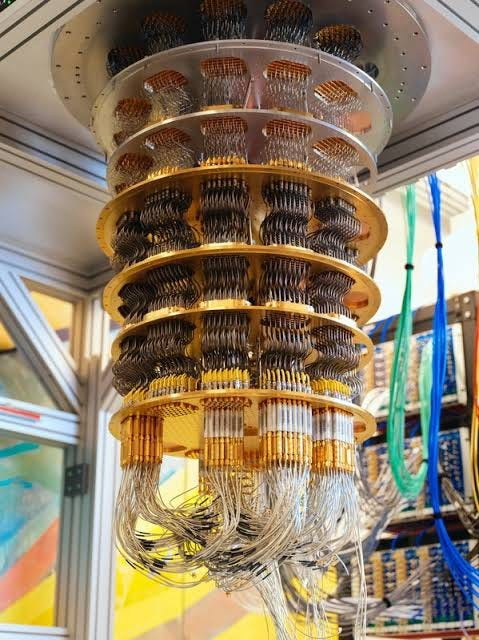
\includegraphics[width=0.4\textwidth]{./slike/quantum_computer1.jpg}
		\caption{Квантни рачунар}
		\label{fig:qc}
	\end{wrapfigure}
	
	Упркос великом напретку, индустрија се суочава са озбиљним техничким препрекама:
	
	\begin{enumerate}
		\item \textbf{Декохеренција:} Кубити су изузетно осетљиви. Чак и најмања промена температуре или електромагнетно зрачење може узроковати губитак квантних својстава (колапс суперпозиције).
		
		\item \textbf{Екстремно хлађење:} Већина данашњих квантних процесора захтева радне температуре близу апсолутне нуле ($-273^{\circ}C$), што чини хардвер гломазним и веома скупим за одржавање.
		
		\item \textbf{Корекција грешака:} Пошто су кубити „шумни”, велики део процесорске снаге троши се на исправљање грешака.
	\end{enumerate}
	
	
	Главни циљ тренутних истраживања је прелазак са NISQ уређаја на Fault-tolerant (отпорне на грешке) квантне рачунаре. Компаније теже ка стварању система са хиљадама логичких кубита који ће моћи да извршавају сложена израчунавања без прекида.
	
	\section{Закључак}
	Утицај квантних рачунара на науку и индустрију је већ сада очигледан, када се узме у обзир невероватна брзина у решавању специфичних проблема (енкрипција, откривање нових лекова и материјала, оптимизација итд.) и могућност симулације природе коју класични рачунари никада неће имати.
	
	Са друге стране, неки од највећих проблема које квантни рачунари доносе су висока цена, огромна потрошња енергије за хлађење и безбедносни ризици по данашњу енкрипцију. Такође, треба нагласити да квантни рачунари нису у свему бољи од класичних рачунара и да не могу решавати све проблеме које може и класични рачунар, већ само специфичне проблеме код којих класични рачунари „ударају у зид”. За једноставније проблеме, проблеме који се решавају при свакодневној употреби класичних рачунара, квантни рачунари нису ефикасни (а нису ни предвиђени за то) и код таквих проблема се класични рачунари показују као бољи.
	
	С тим у вези, можемо претпоставити да будућност не припада искључиво квантним или искључиво класичним рачунарима, већ њиховој хибридној спрези. Очекује се да ће класични суперрачунари користити квантне процесоре (QPU) као специјализоване акцелераторе за најтеже задатке, али да ће у свакодневној употреби и даље бити доминантни класични рачунари. У наредним деценијама, квантна технологија ће вероватно донети револуцију у откривању нових материјала и лекова, као и новом приступу енкрипцији, чиме ће оправдати деценије улагања и теоријског истраживања која су започела Фајнмановом визијом.
	
	\newpage
	
	\phantomsection
	\addcontentsline{toc}{section}{Литература}
	\begin{thebibliography}{9}
		
		\bibitem{wiki_qc} 
		Wikipedia contributors, \textit{Quantum computing}, доступно на: \url{https://en.wikipedia.org/wiki/Quantum_computing}
		
		\bibitem{feynman}
		Richard Feynman, \textit{Simulating Physics with Computers}, International Journal of Theoretical Physics, 1982.
		
		\bibitem{ibm}
		IBM, \textit{What is quantum computing?}, доступно на: \url{https://www.ibm.com/think/topics/quantum-computing}
		
		\bibitem{google}
		Google Quantum AI, \textit{What is Quantum Computing?}, доступно на: \url{https://quantumai.google/whatisqc}
		
	\end{thebibliography} 
	
	
\end{document}